\chapter{Testare}
\pagestyle{headings}

Pentru testarea bibliotecii wxStyle, a'sa cum este cazul cu toate proiectele software, recunoa'stem trei tipuri de testare ce difer'a at{\ia}t prin aria pe care o acoper'a c{\ia}t 'si elementele care sunt testate. Aceste tipuri sunt:

\begin{enumerate}
\item Testarea la nivel de cod - presupune testarea individual'a a componentelor individuale ce alc'atuiesc sistemul 'si formeaz'a infrastructura acestuia. Aceste teste sunt func'tionale 'si trateaz'a componentele ca pe ni'ste cutii negre ale c'aror implementare este irelevant'a. Testele de acest tip sunt automate, ceea ce 'inseamn'a ca pot detecta bug-uri recurente (regression testing) 'si se poate realiza o testare global'a a 'intregului sistem la orice nou' a modificare. Metodologia \emph{Test Driven Development} descrie un proces numit \emph{Red, Green, Refactor} care presupune 'inceperea proiectului prin scrierea de teste ce descriu 'si verific'a func'tionalitatea proiectului. Deoarece aceste teste sunt scrise 'inaintea implement'arii, ele vor pica, adic'a vor fi \emph{Red}. Urm'atorul pas este implementarea func'tionalit'a'tii care determin'a trecerea tuturor testelor, fac{\ia}ndu-le \emph{Green}. Pentru a asigura un cod curat si bine 'intre'tinut, ultimul pas presupune cur'a'tarea 'si rafinarea acestuia prin procesul de \emph{Refactoring}.
\item Testarea la nivel de bibliotec'a - presupune testarea func'tionalit'a'tii 'intregului sistem al bibliotecii. Aceste teste pot fi implementate similar cu cele de la nivelul de cod, dac'a sistemul permite testarea sub form'a de cutie neagr'a.
\item Testarea la nivel de aplica'tie - presupune testarea func'tionalit'a'tii aplica'tiei, presupun{\ia}nd c'a aceasta este alc'atuit'a din componente testate. O aplica'tie ce utilizeaz'a biblioteca wxStyle este implicit o aplica'tie cu interfa't'a vizual'a. Testarea unei astfel de aplica'tii necesit'a simularea interac'tiunii cu utilizatorul 'si interpret'arii rezultatelor afi'sate. De'si exist'a framework-uri ce realizeaz'a aceast'a func'tionalitate pentru biblioteci de interfa't'a precum Java Swing \footnote{https://code.google.com/p/fest/}, biblioteca wxWidgets nu beneficiaz'a de astfel de unelte, iar implementarea lor este una deosebit de dificil'a.\cite{tdddoesntwork}
\end{enumerate}

Scopul proiectului este acela de a realiza o bibliotec'a de obiecte vizuale stilizabile, deci testele la nivel de aplica'tie nu se aplic'a 'in acest context.

\section{Testare la nivel de cod}

Pentru testarea la nivel de cod am utilizat biblioteca \emph{boost::test} pentru a construi unit teste automate, grupate in suite. Spre deosebire de metodologia \emph{Test Driven Development}, am scris testele 'in urma scrierii codului. Testele sunt implementate in proiectul numit \emph{tests} care face parte din solu'tia Visual Studio a proiectului. Un exemplu de test scris cu ajutorul bibliotecii \emph{boost::test} 'il g'asi'ti in figura \ref{fig0601}

\begin{figure}[H]
\begin{lstlisting}[language=C++]
BOOST_AUTO_TEST_CASE(style_loading) {
    XMLStylesheetLoader loader;
    Stylesheet stylesheet = loader.Load("test.xml");
    DefinitionBundle defaultStyle = stylesheet.GetStyle("default").GetBundle(Style::CAT_DEFAULT);
    BOOST_CHECK(defaultStyle.GetBackgroundColor() == "#323335");
}
\end{lstlisting}
\caption{Exemplu de testare al unei componente utiliz{\ia}nd biblioteca \emph{boost::test}}
\label{fig0601}
\end{figure}

Testele din proiectul \emph{tests} acoper'a urm'atoarele componente ale bibliotecii wxStyle:

\begin{itemize}
\item Defini'tiile de stil - sunt testate folosind mijloacele de construire prin cod, iar apoi valorile lor sunt verificate s'a fie egale cu valorile folosite la construire. Se mai testeaz'a 'si opera'tia de combinare (merge) a mai multor defini'tii de stil.
\item Structura \emph{Unified Dimension} - este testat'a prin verificarea valorii calculate din componentele relative 'si absolute este corect'a relativ la o valoare de referin't'a. De asemenea, este testat'a parsarea corect'a a valorilor din reprezentarea de tip string, adic'a a metodei \emph{Dimension::ValueOf(std::string)}. Testele acestei structuri verific'a 'si corectitudinea structurilor \emph{DimPoint} 'si \emph{DimRect}.
\item 'Inc'arcarea fi'sierelor de stiluri - este testat'a verific{\ia}nd rezultatul produs de metoda \emph{XMLStylesheetLoader} asupra unui fi'sier de stiluri de test.
\item 'Inc'arcarea 'si adiministrarea imaginilor - este testat'a utiliz{\ia}nd imagini de test care sunt 'inc'arcate prin clasa \emph{ImageRepository}.
\item Algoritmi - precum calculul offset-ului utiliz{\ia}nd ancore verticale si orizontale sunt testa'ti aplic{\ia}nd algoritmii pe valori predefinite, iar apoi verific{\ia}nd rezultatul acestora 'impotriva rezultatelor a'steptate.
\item Instruc'tiunile de desenare - sunt testate doar prin construc'tia acestora 'si verificarea parametrilor.
\end{itemize}

\section{Testare la nivel de bibliotec'a}

Testarea la nivel de bibliotec'a presupune testarea obiectelor de interfa't'a at{\ia}t din punct de vedere al func'tionalit'a'tii acestora, dar 'si din punct de vedere al prezent'arii lor. Pentru a testa func'tionalitatea obiectelor de interfa't'a, trebuie sa simulam evenimentele produse de utilizator 'si s'a observ'am schimb'arile in starea componentelor 'si evenimentele generate de acestea. Pentru a testa modul de prezentare al obiectelor de interfa't'a, trebuie sa compar'am figura grafic'a a obiectului de interfa't'a cu figura a'steptat'a. Pentru a automatiza ambele moduri de testare presupune efort sporit si investi'tie de timp pe care nu l-am putut aloca. Din acest motiv, testarea la nivel de bibliotec'a se realizeaz'a utiliz{\ia}nd aplica'tia demonstrativ'a.

\begin{figure}[H]
\begin{center}
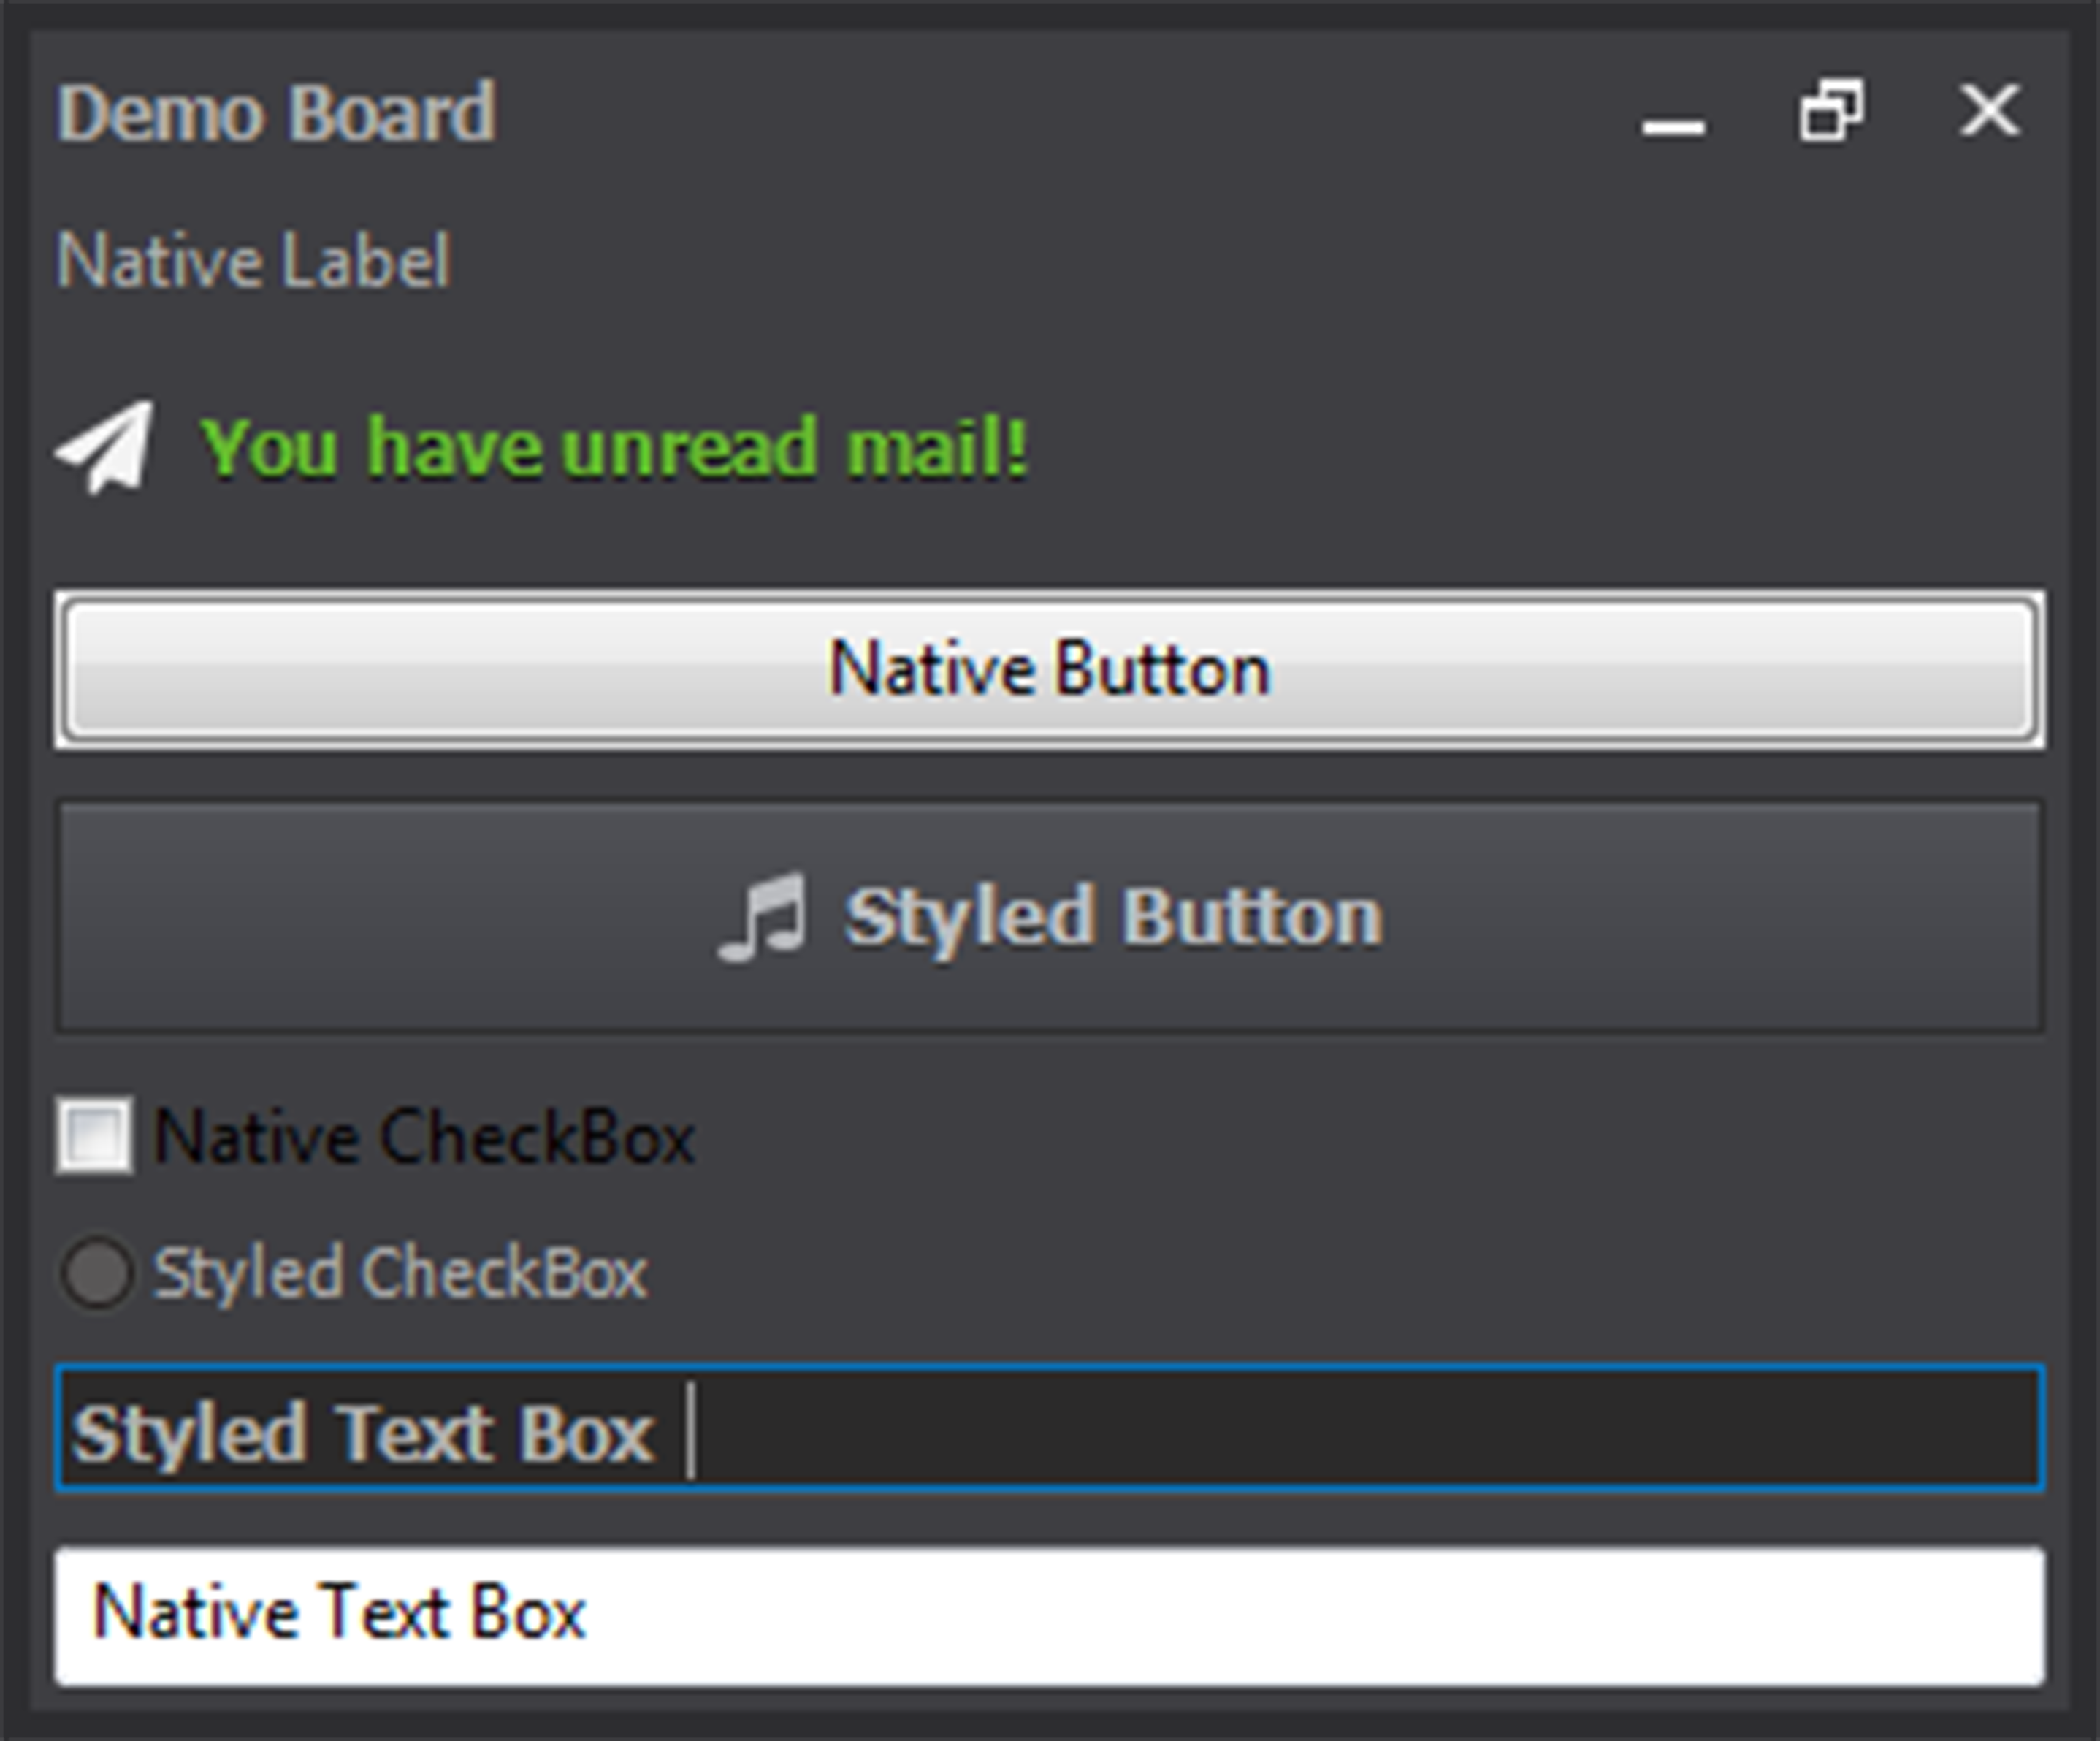
\includegraphics{img/ch6_demo_app.png}
\end{center}
\caption{Captur'a de ecran a aplica'tiei demonstrative}
\label{fig0602}
\end{figure}

Aplica'tia demonstrativ'a con'tine obiecte de interfa't'a stilizabile dar 'si obiecte de interfa't'a din biblioteca wxWidgets. Acestea din urm'a sunt prezente pentru a putea face o compara'tie 'intre modul de prezentare 'si func'tionare al obiectelor stilizabile. Figura \ref{fig0602} prezint'a o captur'a de ecran a aplica'tiei demonstrative.

\medskip

Aplica'tia demonstrativ'a permite urm'atoarele teste:

\begin{itemize}
\item Testarea ferestrei prin posibilitatea de redimensionare 'si mi'scare. Se poate testa manual comportamentul ramei ferestrei, butoanelor de ac'tiune precum minimize, maximize 'si close, 'si aspectul panoului de titlu. Se mai poate testa manual comportamentul panoului de titlu la ac'tiuni de tipul \emph{drag} care trebuie s'a determine mi'scarea ferestrei.
\item Testarea func'tionalit'a'tii obiectelor de interfa't'a. La obiectele de interfa't'a se ata'seaz'a observatori de evenimente care notific'a printr-un dialog de mesaj producerea unui eveniment. 'In acest fel, evenimentele generate de obiectele de interfa't'a sunt semnalate utilizatorului. Se mai poate testa comportamentul acestora la evenimente de intrare precum mi'scarea dispozitivului mouse, ap'as'area de butoane 'si taste, etc. De exemplu, pentur obiectul de interfa't'a StyledTextBox poate fi testat comportamentul la introducerea unui text mai lung dec{\ia}t cutia de text, sele'ctia folosind tastele de navigare, rezultatul ac'tiunilor de stergere asupra unui text vid, etc.
\item Testarea prezent'arii obiectelor de interfa't'a. Prin specificarea, 'in cadrul aplica'tiei demonstrative, unor stiluri, utilizatorul poate verifica modul de prezentare al obiectelor de interfa't'a. Acesta (utilizatorul) poate observa reprezent'arile diferite ale unui obiect 'in func'tie de starea acestuia. De exemplu: modul de prezentare al butonului c{\ia}nd este l'asat liber, c{\ia}nd este acoperit de dispozitivul mouse, c{\ia}nd este ap'asat, etc.
\end{itemize}

De'si mai pu'tin puternic'a dec{\ia}t o alternativ'a automat'a, testarea manual'a utiliz{\ia}nd aplica'tia demonstrativ'a ofer'a posibilitatea compara'tiei 'intre obiectele native wxWidgets, considerate a fi standard, 'si cele stilizabile. Mai mult dec{\ia}t o alternativ'a automat'a, o astfel de testare ii ofer'a utilizatorului posibilitatea test'arii oric{\ia}tor scenarii, intr-un mediu real (fa't'a de unul simulat). O astfel de testare manual'a permite observarea laten'tei 'si a timpului de r'aspuns 'si a artefactelor de desenare. Cu toate acestea este de dorit implementarea unui framework de testare automat'a, pentru a asigura func'tionalitatea corect'a a tuturor elementelor de interfa't'a, f'ar'a a irosi timp de testare manual'a.